

%%%%%%%%%%%%%%%%%%%%%%%%%%%%%%%%%%%%%%%%%%%%%
\graphicspath{{/media/data/Work/cnstellate/golgi/}{/media/data/Work/Responses/}{/media/data/Work/cnstellate/Responses/}{../figures/}{./gfx/}}
%%%%%%%%%%%%%%%%%%%%%%%%%%%%%%%%%%%%%%%%%%%%%

\section[Golgi Cell Model]{Golgi Cell Model: Optimisation using
  monotonic rate-level responses in marginal shell units}
\label{sec:golgi-cell-model}
% Modelling in the auditory periphery has benefited extensively from
% the work of Liberman, Greewood, Patterson, Young, Sachs and others,
% in acoustic \texttt{in vivo} experiments.

\subsection{Background}

The source of GABAergic inputs to cells in the mammalian CN is
somewhat contentious. Despite studies showing that GABAergic inputs to
the CN generally arise in the peri-olivary regions of the medulla in
cats \citep{OstapoffBensonEtAl:1997} and birds
\citep{LachicaRubsamenEtAl:1995,YangMonsivaisEtAl:1999}, slice
preparations of the isolated murine VCN have shown sensitivity to
bicuculine in TS and DS cells \citep{FerragamoGoldingEtAl:1998a}.  The
only known source of GABA intrinsic to the VCN are the golgi cells of
the granule cell domain (GCD) overlying the VCN
\citep[Fig.~\ref{fig:CNdiagram}]{Mugnaini:1985,FerragamoGoldingEtAl:1998}.
The presence of GABAergic inputs to TS, DS and TV cells has been
verified by labeled terminals adjacent to the soma and dendrites
\citep{SmithRhode:1989,AwatramaniTurecekEtAl:2005,BabalianRyugoEtAl:2003}
and release from inhibition in their response areas with
ionotopopheretic application of the \GABAa antagonist, bicuculine
\citep{EvansZhao:1998,CasparyBackoffEtAl:1994,BackoffShadduckEtAl:1999,FerragamoGoldingEtAl:1998a}.

\medskip{}

\yellownote{TODO: Clean up paragraph}
Other studies in the rat cochlear nucleus relating to the Golgi cell or GABA:
\begin{itemize}
\item \citep{MugnainiOsenEtAl:1980} Fine structure of granule cells
  and related interneurons (termed {Golgi} cells) in the cochlear
  nuclear complex of cat, rat and mouse
\item GABAa expression in the rat brainstem  \citep{CamposCaboEtAl:2001}
\item \citep{Alibardi:2003a} Ultrastructural distribution of
  glycinergic and {{GABAergic}} neurons and axon terminals in the rat
  dorsal cochlear nucleus, with emphasis on granule cell areas
\item \citep{AwatramaniTurecekEtAl:2005} Staggered {Development} of
  {GABAergic} and {Glycinergic} {Transmission} in the {MNTB}
\end{itemize}

\medskip{}

\yellownote{TODO: Expand role of GABA, or combine with previous para}
Role of GABA in the VCN
\begin{itemize}
\item Effects of microiontophoretically applied glycine and {GABA} on
  neuronal response patterns in the cochlear nuclei
  \citep{CasparyHaveyEtAl:1979}
\end{itemize}

\citep{Alibardi:2003a} rat CN complex -> Golgi-stellate cells
(fusiform layer: 2) in DCN contact granule and unipolar brush cells

\medskip{}

Inputs to golgi cells are more complicated than VCN cells in the core
regions. Golgi cells are sparse in the GCD, surrounded by the many,
smaller excitatory granule cells, that form small en passant
endings. Type II ANFs create diffuse glutamatergic release sites in
the GCD \citep{HurdHutsonEtAl:1999,BensonBrown:2004} that may
stimulate NMDA glutamate receptors in golgi cells
\citep{FerragamoGoldingEtAl:1998a}.

\medskip{}

Extracellular recordings from the GCD by \citet{GhoshalKim:1997}, are
most likely from golgi cells since granule cell somata are less than
$10 \mu m$ and very narrow axons. The majority of recorded units
showed a monotonic increase in firing rate with increasing sound
intensity \citep{GhoshalKim:1997}.

\medskip{}

The known GABAergic input to VCN units comes primarily from the
superior olive (ref), but the presence of active GABA synapses in
isolated VCN slices by \citet{FerragamoGoldingEtAl:1998} led to
further investigation of golgi cells in the granule cell
domain. \citet{FerragamoGoldingEtAl:1998a} showed that golgi cells
have a classic type-I current response, which suggest they integrate
inputs, and their response to AN shocks were delayed by approximately
0.7~ms relative to the core VCN units .  Ghosal and Kim
\citet{GhoshalKim:1997} examined the VCN marginal shell in cats
(equivalent to the GCD in mice) that golgi cells provide some sort of
automatic gain control to the principle VCN units, through their
monotonic responses to tones and noise.

\medskip{}

% (Reference) showed that in adult animals high-spontaneous rate ANFs do not
% project to the GCD; they do show that low-spontaneous rate ANFs do project into
% the GCD, albeit more profusely than in the core on the VCN.
   

\begin{figure}[htb]
  \centering
\resizebox{0.8\textwidth}{!}{\includegraphics{NoFigure}}
%  \resizebox{0.8\textwidth}{!}{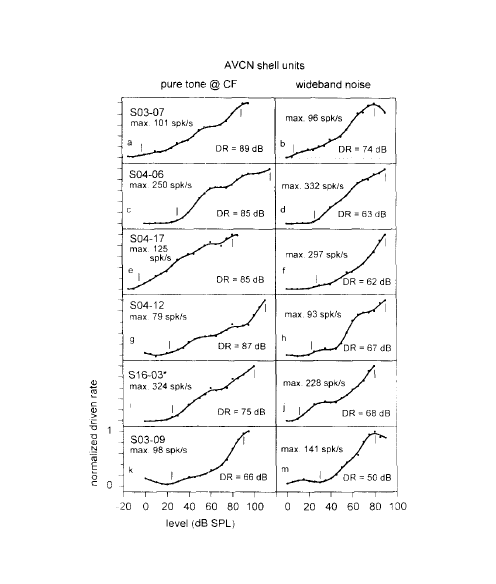
\includegraphics{GhoshalKim}}
\caption{Rate level response of unit S03-07 (CF 21~kHz) from Fig2
  \citep{GhoshalKim:1997} }
\end{figure}


\newpage
\subsection{Implementation}

In the creation of the golgi cell model, we can reduce the explicit
responses of Golgi cells down to three major details: a) golgi cells are integrators due to their type-I~current clamp response, b) golgi cells are (most likely) monotonic to tone and noise rate increases, and
c) they have a significant delay of first spike latency relative to the core VCN units. The lack of extensive experimental data meant that a Poisson rate neural model
would be preferred over the Hogkin-Huxley type neural model. 

\medskip{}

In Chapter~\ref{sec:GAChapter} and previous publications \citep{EagerGraydenEtAl:2006a}, the golgi cell model was implemented as a single-compartment conductance  neuron. Due to the unavailability of sufficient data regarding \emph{in vivo}
golgi cell responses, we have decided to simulate the response of
golgi cells using inputs from the auditory model's instantaneous rate outputs rather
than simulating the neural membrane with Hodgkin-Huxley models.  A number of steps
were taken to investigate the golgi cell model (a further detailed explanation is in the chapter Appendix~\ref{sec:chp3appendix}).

\medskip{}

Monotonic rate-level data from GCD in VCN \citep{GhoshalKim:1996} unit
S03-07 (CF 21~kHz) was used to optimise parameters ${\rm
golgi\_spon}$, \wLSRGLG, \wHSRGLG, and \sANFGLG\@.  The optimisation
method was a default using the principle-axis method.

\medskip{}

Due to its replication of granule cells in the model, weight for LSR \wLSRGLG and HSR \wHSRGLG are determined for all synapses, number \nLSRDS and \nHSRDS, delay \dANFGLG added to smoothing function to ensure conductance and dendritic filtering are included.

\subsubsection{Key design factors}
\yellownote{TODO: expand para, include fig ref} - Choosing neural model: HH-type or Poisson
 - Problem of monotonic excitation at low level
  - added HSR to model to avoid added computation of MSR
 - Spread of ANF to GCD ARE broader than core VCN
  - are we spoiling the broth too early? 


\begin{figure}[hp!]
  \centering
  \includegraphics[width=0.9\textwidth,trim=0 110mm 1 55mm]{gfx/GolgiDiagram}
  \caption{ The golgi instantaneous-rate profile was generated using ANF
    profiles. $\mu$ and $\sigma$ control the spread of connections
    across frequency channels, and $\mathbf{w}$ is
    the weighted sum of HSR and LSR instantaneous-rate vectors,
    $\alpha$ is the synaptic and dendritic smoothing function.}
\end{figure}

\yellownote{TODO: explain the tables below}
{%
\small\linespread{0.5}
\noindent%
\begin{table}[!thb]
    \caption{Golgi cell model summary (Nordlie format)}
    \label{tab:GolgiCellModelSummary}
\begin{tabularx}{\textwidth}{|l|X|} %
\hdr{2}{A}{Model Summary}\\
%\begin{ntab}{|l|X|}{2}{\ref{tab:GolgiCellModelSummary} A}{Model Summary}\\\hline
 \textbf{Populations}  & ANF~(HSR, LSR) and Golgi (GLG) cells \\\hline 
  \textbf{Topology}    & Tonotopic - 100 frequency channels (0.2--40
  kHz);  Cat model; Greenwood function centre frequencies \citep{Greenwood:1990}\\\hline
\textbf{Connectivity}  & ANF to GLG filter inputs, Gaussian spread
centred on channel\\\hline
\textbf{Input model}  & ANF~model: Version 4 and 5 Zilany model \citep{ZilanyBruce:2007,ZilanyBruceEtAl:2009} \\\hline
\textbf{Neuron model}  & GLG cell model: Instantaneous-rate Poisson
neuron model \\\hline
\textbf{Synapse model} & Synapto-dendritic smoothing filter (alpha function) \\\hline
%    \textbf{Input}     & Pure tones (22.7 kHz, 50 ms, 5 ms on/off ramp, 20 ms delay), intensity range 0--100 dB~SPL   \\\hline
%\textbf{Measurements}  & Mean firing rate of Golgi cell instantaneous rate profile or PSTH sampled from Poisson spike-generator (25 repetitions) \\\hline
\end{tabularx}
\vspace{1ex}
%\end{ntab}

% - B ------------------------------------------------------------------------
\noindent%
\begin{tabularx}{\textwidth}{|l|X|X|}%
\hdr{3}{B}{Populations}\\
\textbf{Name} &                         \textbf{Elements}                          & \textbf{Number} \\\hline
     HSR      & Auditory nerve fibre model
     \citep{ZilanyBruce:2007,ZilanyBruceEtAl:2009} & Rate models only,
     1 per channel\\\hline
     LSR      & Auditory nerve fibre
     \citep{ZilanyBruce:2007,ZilanyBruceEtAl:2009} & Rate models only,
     1 per channel \\\hline
     GLG      &                 Instantaneous-rate Poisson neuron model                  & 1 unit (CF 22.7 kHz, channel 76)  \\\hline
\end{tabularx}
\vspace{1ex}

% - C ------------------------------------------------------------------------------
\noindent
\begin{tabularx}{\textwidth}{|l|l|l|X|}%
\hdr{4}{C}{Connectivity}    \\
     \textbf{Name}       & \textbf{Source} & \textbf{Target} & \textbf{Pattern} \\\hline
\multirow{2}{*}{\ANFGLG} &     {\HSR}      &      GLG      & 
Gaussian spatial convergence, centred on CF, spread parameter
(\sHSRGLG = 2). Weight (\wHSRGLG) to be optimised. \\
   &     {\LSR}      &      GLG      & 
Gaussian spatial convergence, centered on \CF.  Spread (\sLSRGLG) and weight (\wLSRGLG) to be optimised. \\\hline
\end{tabularx}
\vspace{1ex}
% - D ------------------------------------------------------------------------------
\noindent%
\begin{tabularx}{\linewidth}{|p{0.22\linewidth}|X|}
\hdr{2}{D}{Neuron and Synapse Model}\\
 \textbf{Name} & Golgi cell model \\\hline
 \textbf{Type} & Instantaneous-rate Poisson neural  model \\\hline 
%\raisebox{-4.5ex}{\parbox{\linewidth}{\textbf{Model Dynamics}}} & 
 \textbf{Model Dynamics} & %
% {\rule{1em}{0em}\vspace*{-1.5ex}\scriptsize%
% \begin{equation*}%
%  \begin{array}{r@{\;=\;}ll}
%   \mathbf{w}_{L,H}&  w_{LSR,HSR \to GLG}\,\mathcal{N}(i_{{\rm CF}},\sigma)    & \text{Gaussian weight mean at CF, \sigma^2=\sLSRGLG} \\ 
%   \alpha(t)      &\left( t  \exp(\frac{-t}{\Gtau}) \right)   &  \text{Synapto-dendritic filter with unit area} \\
%   g(t)           & \mathbf{w}_{L}\bullet\mathbf{L}+\mathbf{w}_{H}\bullet\mathbf{H} & \text{Sum of dot products} \\ % between weights and ANF rate matrices}\\ 
% %\mathbf{H},\mathbf{L} \to f(\text{channel},t) & \mathbf{w}_{H,L} \to f(\text{channel})\\
%              %      r(\mathbf{x})              &               \max\{\mathbf{x}(t-\dANFGLG) - x(0) + \Gspon,0\}                & \\
%  G(t)  &   \lfloor \, \alpha(t)\,\ast\,g(t) \,\rfloor                  & \text{Convolution of $\alpha(t)$ and $g(t)$ and rectification}\\
% % & \text{if } G(t) < 0 \,G(t)=0 & \text{rectification of Golgi model rate} \\
% \end{array} \end{equation*}\vspace*{-1.5ex}\rule{1em}{0em}}  \\\hline
%{\rule{1em}{0em}\vspace*{-1.5ex}%\scriptsize%
See Figure~\ref{fig:GolgiDiagram} and the GLG rate filter model
Equations~\ref{eq:GolgiWeights}--\ref{eq:GolgiConvolution}.
% ($g_{i}(t)$) used for
% the Golgi cell model. It was created using convolution of weighted ANF input rates
% and synapto-dendritic kernel ($\alpha_{\small\rm GLG}(t)$) with rectification. 
% \begin{equation*}%
%  \begin{array}{r@{\;=\;}l}
%  {\rm GLG}_{i}(t)  &  \alpha_{\rm GLG}(t)\,\ast\,g(t) \,\rfloor + \text{SR}_{\rm GLG} \quad \text{where} \\
%   \alpha(t)      &\left( t  \exp(\frac{-t}{\Gtau}) \right)   \quad  \text{and} \\
%   g(t)           & \mathbf{w}_{L}\bullet\mathbf{L}+\mathbf{w}_{H}\bullet\mathbf{H} 
% \end{array} \end{equation*}\vspace*{-1.5ex}\rule{1em}{0em}
%Preliminary rate, $g(t)$, is the sum of dot products between weight vectors and ANF rate matrices.
% Gaussian weight vectors have mean at CF and $\sigma^2=\sLSRGLG$.}  
\\\hline
 \textbf{Spiking} & Renewal Poisson process given instantaneous rate, ${\rm GLG}_{i}(t)$,  with refractory effects  \citep{ZilanyBruce:2007,Jackson:2003} \\\hline
\end{tabularx}
\vspace{2ex} 

% $\dag$\footnotesize{Synaptic filter, $\alpha(t)$, is normalised, by setting the
%   area under the alpha function to one. For a large enough filter length, the
%   alpha function integral ($\int \alpha(t) dt = (-\Gtau^2 - t \cdot \Gtau)\cdot
%   \exp(-\frac{t}{\Gtau})$) approximately equals $\Gtau^2$. In this case $10
%   \times \Gtau$ is used for the filter length.}  

% - E -----------------------------------------------------------------------------
\noindent
\begin{tabularx}{\linewidth}{|l|X|} %
\hdr{2}{E}{Optimisation}\\
\textbf{Input Stimulus} & Rate Level function, 22.7~kHz tone at SPL -15 to 90 dB (50 ms duration, 2 ms cosine squared on\slash off ramp, 20 ms delay)\\\hline 
\textbf{Parameters} & 
 \sANFGLG, 
   \Gtau,   
 \wHSRGLG,  
 \wLSRGLG,  
  \Gspon   \\\hline
\textbf{Fitness function}  & RMS squared error between rate-level functions of Golgi model (channel 76, CF=22.7 kHz) and unit S03-07 (CF=21 kHz) from \citet{GhoshalKim:1996}. Mean rate of Golgi model spikes sampled from 25 repetitions. \\\hline
\end{tabularx}
\vspace{1ex}
% \begin{ntab}{4}{|X|c|c|c|}{E}{Optimisation NTAB}
% \textbf{Parameters}             &    \textbf{Name}     & \textbf{Range} & \textbf{Best Values} \\\hline 
%  Spatial spread $\ANFGLG$ (channel unit)   &      $\sANFGLG$      &     [0,10]     & 2.48  \\\hline 
%  Synaptodendritic filter time constant (ms)     &   $\tau_{\ANFGLG}$     &     [0,20]       & 5.01  \\\hline 
%       Weighted sum of HSR (unitless)       &      $\wHSRGLG$      &     [0,5]      & 0.517 \\\hline 
%       Weighted sum of LSR (unitless)       &      $\wLSRGLG$      &     [0,5]      & 0.0487\\\hline 
% Golgi spontaneous rate (spikes per second) & \texttt{golgi\_spon} &     [0,50]     & 3.73  \\\hline
% \end{ntab}
\end{table}%
}

%%% Local Variables: 
%%% mode: latex
%%% TeX-master: "SimpleResponses"
%%% TeX-PDF-mode: nil
%%% End: 




% \includegraphics[width=0.6\textwidth,angle=-90]{GolgiRateLevelActualFit}\\
% \caption{Optimisation Results for Golgi Model using Rate Level data
%   from }\label{Ch3:fig:GolgiFit}
% \includegraphics[width=0.8\textwidth]{GolgiRateLevel}\\
% \caption{Optimisation Results for Golgi Model using Rate Level data
%   from }\label{Ch3:fig:GolgiRL}

% \includegraphics[width=0.8\textwidth]{golgi_RateLevel_opt}\\
% \caption{Optimisation Results for Golgi Model using Rate Level data
%   from }\label{Ch3:fig:GolgiRL}
% \includegraphics[width=0.8\textwidth,angle\todo=-90]{GolgiRateLevel2}\\
% \caption{Optimisation Results for Golgi Model using Rate Level data
%   from }\label{Ch3:fig:GolgiRL}

\clearpage
\subsection{Results}


Golgi model (Green) and spike based output (Pink) was used to
fit the experimental data of unit S03-07 (CF 21~kHz) from
\citep{GhoshalKim:1996} (Red).  LSR mean rate (Blue) of 21~kHz unit is
monotonic with a high threshold.

\yellownote{TODO: expand results output}
Figure \ref{fig:golgiresults} shows the output of the optimised golgi cell model.
\textbf{Error} 0.021 (MSE re max rate)


\begin{figure}[htb]
  \centering %\turnbox{90}{\small{Rate (sp/s)}}
  \resizebox{0.7\textwidth}{!}{\includegraphics[angle=-90]{GolgiRateLevel-2}}\\
  \caption{Golgi cell model optimisation results with the best response obtaining a minimum error 0.021 (spikes/s, average mean squared error of experimental and data points). }\label{fig:golgiresults}
\end{figure}


%   % \includegraphics[width=0.6\textwidth,angle=-90]{GolgiRateLevelActualFit}\\
%   % \caption{Optimisation Results for Golgi Model using  Rate Level data from }\label{Ch3:fig:GolgiFit}
%   % \includegraphics[width=0.8\textwidth]{GolgiRateLevel}\\
%   % \caption{Optimisation Results for Golgi Model using  Rate Level data from }\label{Ch3:fig:GolgiRL}

%   % \includegraphics[width=0.8\textwidth]{golgi_RateLevel_opt}\\
%   % \caption{Optimisation Results for Golgi Model using  Rate Level data from }\label{Ch3:fig:GolgiRL}
%   % \includegraphics[width=0.8\textwidth,angle=-90]{GolgiRateLevel2}\\
%     % \caption{Optimisation Results for Golgi Model using  Rate Level data from }\label{Ch3:fig:GolgiRL}





% \begin{figure}[htb]
% \centering
%   \includegraphics[width=0.6\textwidth,angle=-90]{GolgiRateLevelActualFit}\\
%   \caption{Optimisation Results for Golgi Model using  Rate Level data from }\label{Ch3:fig:GolgiFit}
% \end{figure}

% \begin{figure}[htb]
% \centering
%   \includegraphics[width=0.8\textwidth]{GolgiRateLevel}\\
%   \caption{Optimisation Results for Golgi Model using  Rate Level data from }\label{Ch3:fig:GolgiRL}
% \end{figure}

% \begin{figure}[htb]
% \centering
%   \includegraphics[width=0.8\textwidth]{golgi_RateLevel_opt}\\
%   \caption{Optimisation Results for Golgi Model using  Rate Level data from }\label{Ch3:fig:GolgiRL}
% \end{figure}

% \begin{figure}[htb]
% \centering
%   \includegraphics[width=0.8\textwidth,angle=-90]{GolgiRateLevel2}\\
%   \caption{Optimisation Results for Golgi Model using  Rate Level data from }\label{Ch3:fig:GolgiRL}
% \end{figure}





% \clearpage \newpage
\section{Verification}
 \subsection{Tone Response}

% \begin{figure}[h]
%   \centering\resizebox{0.95\textwidth}{!}{%
%     \includegraphics{RateLevel/psthsingle90.3.eps}%
%     \includegraphics{RateLevel/G_ratelevel.eps}}
% \end{figure}
% \begin{figure}[h]
%   \centering\resizebox{0.95\textwidth}{!}{%
%     \includegraphics{RateLevel/response_area.3.eps}%
%     \includegraphics{RateLevel/response_area_log2.3.eps}}
% \end{figure}
% \begin{figure}[h]
%   \centering\resizebox{0.95\textwidth}{!}{%
%     % \includegraphics{RateLevel/response_area.3.eps}
%     \includegraphics{RateLevel/psthall90.3.eps}%
%     \includegraphics{RateLevel/psthVlevel.3.eps}}
% \end{figure}



% \clearpage
 \subsection{Noise Response}
% \begin{figure}[h]
%   \centering\resizebox{0.95\textwidth}{!}{%
%     \includegraphics{NoiseRateLevel/psthsingle120.3.eps}%
%     \includegraphics{NoiseRateLevel/G_ratelevel.eps}}
% \end{figure}
% \begin{figure}[h]
%   \centering\resizebox{0.95\textwidth}{!}{%
%     \includegraphics{NoiseRateLevel/response_area.3.eps}%
%     \includegraphics{NoiseRateLevel/response_area_log2.3.eps}}
% \end{figure}
% \begin{figure}[h]
%   \centering\resizebox{0.95\textwidth}{!}{%
%     % \includegraphics{RateLevel/response_area.3.eps}
%     \includegraphics{NoiseRateLevel/psthall90.3.eps}%
%     \includegraphics{NoiseRateLevel/psthVlevel.3.eps}}
% \end{figure}


% \clearpage
 \subsection{Masked Noise and Tone}
% \begin{figure}[h!]
%   \centering\resizebox{0.95\textwidth}{!}{\includegraphics{MaskedRateLevel/psthsingle90.3.eps}\includegraphics{MaskedRateLevel/G_ratelevel.eps}}
% \end{figure}
% \begin{figure}[h!]
%   \centering\resizebox{0.95\textwidth}{!}{%
%     \includegraphics{MaskedRateLevel/response_area.3.eps}%
%     \includegraphics{MaskedRateLevel/response_area_log2.3.eps}}
% \end{figure}

% \begin{figure}[h!]
%   \centering\resizebox{0.95\textwidth}{!}{%
%     % \includegraphics{RateLevel/response_area.3.eps}
%     \includegraphics{MaskedRateLevel/psthall90.3.eps}%
%     \includegraphics{MaskedRateLevel/psthVlevel.3.eps}}
% \end{figure}
% \clearpage
 \subsection{Masked Response Area}
% \begin{figure}[h!]
%   \centering\resizebox{0.95\textwidth}{!}{%
%     \includegraphics{MaskedResponseCurve/psthsingle5810.3.eps}%
%     \includegraphics{MaskedResponseCurve/G_masked.eps}}
% \end{figure}
% \begin{figure}[h!]
%   \centering\resizebox{0.95\textwidth}{!}{%
%     \includegraphics{MaskedResponseCurve/response_area.3.eps}%
%     \includegraphics{MaskedResponseCurve/response_area_log2log2.3.eps}}
% \end{figure}

% \begin{figure}[h!]
%   \centering\resizebox{0.95\textwidth}{!}{%
%     % \includegraphics{RateLevel/response_area.3.eps}
%     \includegraphics{MaskedResponseCurve/psthall5810.3.eps}%
%     \includegraphics{MaskedResponseCurve/psthVmod.3.eps}}
% \end{figure}
% \clearpage


% \todo{add stuff here}



% % %%%%%%%%%%%%%%%%%%%%%%%%%%%%%%%%%%%%%%%%%%%%%%%%%%%%%%
% \bibliographystyle{plainnat}%bmc_article} % Style BST file
% \bibliography{../manuscript/bib/MyBib}
 
% \end{document}





%%% Local Variables: 
%%% mode: latex
%%% TeX-master: "SimpleResponses"
%%% TeX-PDF-mode: nil
%%% End: 
